\chapter{Analytic Solutions to the Neutron Diffusion Equation}

\section{Introduction}
  The following is a manufactured solution designed for 1D and 2D Finite Element 
  Method (FEM) solvers in one and two spatial dimensions. Multigroup 
  problems are also addressed with a simplified one-dimensional problem.
  
  For the reference problems, the one-group neutron diffusion problem is written
  below.
  \begin{equation} \label{eq:onegroup}
    -D \nabla^2 \phi + \Sigma_r \phi =  \frac{1}{k_{eff}} \nu \Sigma_f \phi + 
      q_{fixed}
  \end{equation}
  For two-group neutron diffusion problems, the two-group neutron diffusion 
  problem is written below.
  \begin{align} 
    -D_1 \nabla^2 \phi_1 + \Sigma_{r1} \phi_1 &= \frac{1}{k_{eff}} \left(
      \nu \Sigma_{f1} \phi_1 + \nu \Sigma_{f2} \phi_2 \right) \\
    -D_2 \nabla^2 \phi_2 + \Sigma_{r2} \phi_2 &= 
      \Sigma_{s 1 \rightarrow 2} \phi_2
  \end{align}
  Where $\phi_1$ is the higher energy group and $\phi_2$ is the lower energy 
  group. This formulation assumes all fission neutrons are created in the fast 
  energy group and there is no up-scattering (scattering that results in an 
  increase in neutron energy). These are realistic assumptions for all diffusive
  neutron systems.

  Analytic solutions for 1D and 2D problems are provided below. These can be 
  replicated in a 2D FEM solver using a square geometry. The reference square is 
  $[0,1]\times[0,1]$. For one-dimension, two of the boundary conditions are set
  to reflective conditions and two to essential $(\phi = 0)$ conditions. For 
  two-dimension, all of the boundary conditions are set to essential conditions.
  
  These formula are common but this specific formulation comes from E. E. Lewis
  \textit{Fundamentals of Nuclear Reactor Physics}.

\section{One Dimension, One-Group, Fixed Source}
  For this problem, the following one-group coefficients are used.
  \begin{align*}
    D &= 1\\
    \Sigma_r &= 1\\
    \nu \Sigma_f &= 0\\
    q_{fixed} &= 1
  \end{align*}
  Then, equation \eqref{eq:onegroup} is written
  \begin{equation}
    - \nabla^2 \phi + \phi = 1 
  \end{equation}
  or
  \begin{equation} \label{eq:diffusion_simplified}
    \nabla^2 \phi - B^2 \phi = S
  \end{equation}
  where $B = 1$ and $S=-1$.
  The solution is composed of a particular and general solution.
  \begin{equation}
    \phi = \phi_g + \phi_p 
  \end{equation}
  For problems of the form of \eqref{eq:diffusion_simplified} the general 
  solution has the form
  \begin{equation} \label{eq:general}
    \phi_g = c_1 \cosh(Bx) + c_2 \sinh(Bx)
  \end{equation}
  And for constant $S=1$, the particular solution has the form
  \begin{align} \label{eq:particular}
    \phi_p &= -S/B \\
    \nonumber &= 1
  \end{align}
  Then, the solution has the form
  \begin{equation} 
    \phi = c_1 \cosh(Bx) + c_2 \sinh(Bx) + 1
  \end{equation}
  The only problem remaining is to solve for $c_1$ and $c_2$. These are given
  by the zero flux boundary conditions at the problem boundaries.
  \begin{align}
    \phi(0) &= 0\\
    \phi(L) &= 0
  \end{align}
  Evaluating the solution at 0, 
  \begin{align}
    \phi(0) &= 0 \\
    &= c_1 + 1\\
    c_1 &= -1
  \end{align}
  Evaluating the solution at $L$
  \begin{align}
    \phi(L) &= 0\\
    &= c_2 \sinh(BL) - \cosh(BL)-1\\
    c_2 &= \frac{\cosh(BL)-1}{\sinh(BL)}
  \end{align}
  The final solution is 
  \begin{equation} \label{eq:one_dimension}
    \phi(x) = -\cosh(Bx) + \frac{\cosh(BL)-1}{\sinh(BL)} \sinh(Bx) +1
  \end{equation}
  
\section{One Dimension, One Group, Criticality} \label{sc:onegroup1d}
  This problem also uses the one-group neutron diffusion equation from 
  \eqref{eq:onegroup} and the following coefficients:
  \begin{align*}
    D &= 1\\
    \Sigma_r &= 1\\
    \nu \Sigma_f &= 2\\
    q_{fixed} &= 0
  \end{align*}
  The problem is then proposed as 
  \begin{equation}
    -\nabla^2 \phi - \phi = 0 
  \end{equation}
  and has general solution
  \begin{equation}
    \phi_g = c_1 \cos(x) + c_2 \sin(x)
  \end{equation}
  and $c_1 = 0 $ for the given boundary conditions yielding
  \begin{equation} \label{eq:sinshape}
    \phi_g = c_2 \sin(x)
  \end{equation}
  The problem is an eigenvalue problem and has infinite solutions so the 
  constant $c_2$ is arbitrary and $\sin(x)=0$. Therefore, the geometric 
  bucking is $1/b$ where $b$ is the characteristic length of the problem. 
  Therefore, the solution is 
  \begin{equation} \label{eq:onedimensionsol}
    \phi = \sin(x/b)
  \end{equation}
  Plugging this solution back into \eqref{eq:onegroup} and dividing both sides
  by $\sin(x/b)$ will yield an expression for $k_{eff}$.
  \begin{align}
    -D B^2 + \Sigma_r &= \frac{1}{k_{eff}} \nu \Sigma_f \\
    k_{eff} &= \frac{\nu \Sigma_f}{DB^2 + \Sigma_r} \label{eq:keff1d}
  \end{align}
  Then, for a slab of length 100 cm, $B = \pi / 100$ and
  \[ k_{eff} = 1.9980280254 \]
\section{Two Dimension, One Group, Criticality}
  The same material coefficients are used for this problem as in the 
  one-dimensional problem. Similar to the one-dimensional problem, this 
  problem has basic solution of $\sin(x/b)$. The problem is separable in the 
  two spatial dimensions. 
  \begin{equation}
    \phi(x,y) = X(x) Y(y) 
  \end{equation}
  Beginning with equation \eqref{eq:onegroup}.
  \begin{align}
    -D \nabla^2 \phi(x,y) + \Sigma_r \phi(x,y) &= \nu \Sigma_f \phi(x,y) \\
    - \nabla^2 \phi(x,y) - \phi(x,y) &= 0 \\
    \nabla^2 \phi(x,y) + \phi(x,y) &= 0 \\
    \frac{\partial^2}{\partial x^2} \phi(x,y) + 
      \frac{\partial^2}{\partial y^2} \phi(x,y) +
      \phi(x,y) &= 0\\
    Y(y)\frac{\partial^2}{\partial x^2}X(x) +
      X(x) \frac{\partial^2}{\partial y^2} Y(y) + X(x)Y(y) &= 0\\
    Y(y)\left(\frac{\partial^2}{\partial x^2}X(x) + \frac{1}{2} X(x)\right)+
      X(x)\left(\frac{\partial^2}{\partial y^2}Y(y) + \frac{1}{2}Y(y)
      \right) &= 0
  \end{align}
  The solution to this problem is the product of the solutions from the 
  previous problem presented in \eqref{eq:onedimensionsol}. The solution is
  \begin{equation} \label{eq:twodimensionsol}
    \phi(x,y) = \sin(x/b) \sin(y/a)
  \end{equation}
  Where $b$ is the x-dimension of the problem and $a$ is the y-dimension of 
  the problem.
  If $B_x=B_y$; that is, $a=b$,  $k_{eff}$ can be calculated as
  \begin{equation}
    k_{eff} = \frac{\nu \Sigma_f}{2DB^2 + \Sigma_r} 
  \end{equation}
  Then, for $a = b = 100$
  \[ k_{eff} = 1.9960599356 \]
\section{One Dimension, Two Group, Criticality}
  Much of this section is drawn from a manuscript prepared by Dr. Scott 
  Palmtag \textit{Analytic Solution to 2-group Bare Core Problem}, June 2018.
  
  A two-group neutron diffusion problem is considered for a one-dimensional
  homogeneous slab. Energy group 1 is higher energy than energy group 2. 
  Regarding the energy structure, it is assumed all fission neutrons are 
  produced in the fast group (i.e. $\chi_1=1$ and $\chi_2=0$). Additionally, 
  it is assumed that there is no up-scattering 
  (i.e. $\Sigma_{2\rightarrow1}=0$).
  
  Then, the two-group neutron diffusion equations are given in \eref{eq:}
  \begin{align} \label{eq:twogroup}
  \begin{split}
    -D_1 \nabla^2 \phi_1 + \Sigma_{r1} \phi_1 &= \frac{1}{k_{eff}} \left(\nu 
      \Sigma_{f1} \phi_1 + \nu \Sigma_{f2} \phi_2 \right) \\
    -D_2 \nabla^2 \phi_2 + \Sigma_{r2} \phi_2 &= \Sigma_{s1\rightarrow2} 
      \phi_1 
  \end{split}
  \end{align}
  
  Referring to the problem posed by Section \ref{sc:onegroup1d}, the flux 
  solutions have form given in equation \eqref{eq:sinshape}. Then
  \begin{align} \label{eq:twogroupflux}
  \begin{split}
    \phi_1 &= c_1 \sin(Bx) \\
    \phi_2 &= c_2 \sin(Bx)
  \end{split}
  \end{align}
  Where $B$ is the geometric buckling term. For this geometry, the geometric 
  buckling of the fundamental mode is given by 
  \begin{equation}
    B = \pi/L
  \end{equation}
  where $L$ is the length of the problem. Then, plugging 
  \eqref{eq:twogroupflux} into the second equation from \eqref{eq:twogroup} 
  and dividing the equation by $\sin(Bx)$
  \begin{equation}
    D_2 B^2 c_2 + \Sigma_{r2} c_2 = \Sigma{s1\rightarrow2} c_1
  \end{equation}
  Then, the ratio can be expressed
  \begin{equation} \label{eq:fluxratio}
    \frac{c_2}{c_1} = \frac{\Sigma_{s1\rightarrow2}}{D_2 B^2 + \Sigma_{r2}}
  \end{equation}
  Returning to the first equation from \eqref{eq:twogroup} and again dividing
  both sides by $\sin(Bx)$
  \begin{align}
    D_1 B^2 c_1 &= \frac{1}{k_{eff}} \left( \nu \Sigma_{f1} c_1 + 
      \nu \Sigma_{f2} c_2\right)\\
    k_{eff} &= \frac{\nu \Sigma_{f1} c_1 + \nu \Sigma_{f2} c_2}
      {D_1 B^2 c_1 + \Sigma{r1} c_1}\\
    k_{eff} &= \frac{\nu \Sigma_{f1} + \nu \Sigma_{f2} c_2/c_1}
      {D_1 B^2 + \Sigma{r1}}
  \end{align}
  Plugging in the expression from \eqref{eq:fluxratio}
  \begin{equation}
    k_{eff} = \frac{\nu \Sigma_{f1} + \nu \Sigma_{f2} 
      \left(\frac{\Sigma_{s1\rightarrow2}}{D_2B^2+\Sigma_{r2}}\right)}
      {D_1 B^2 + \Sigma{r1}}
  \end{equation}
  From the VVER-440 benchmark, material 1,
  \begin{align*}
    D_1 &= 1.3466  \\
    D_2 &= 0.37169 \\
    \Sigma_{r1} &= 2.5255\text{E}-2\\
    \Sigma_{r2} &= 6.4277\text{E}-2\\
    \nu \Sigma_{f1}  &= 4.4488\text{E}-3\\
    \nu \Sigma_{f2}  &= 7.3753\text{E}-2\\
    \Sigma_{s1\rightarrow2} &= 1.6893\text{E}-2 \\
    k_{\infty} &= 0.943664259
  \end{align*}
  For a 100cm slab then,
  \begin{align*}
    \frac{c_2}{c_1} &= 0.26132419 \\
    k_{eff} &= 0.892349025
  \end{align*}
\section{One-Dimension, One-Group, Two-Region, ``Reactor''}
  This final analytic problem was designed to test the materials mapping of a
  FEM solver. The problem is proposed as a slab-reactor with a fuel and 
  reflector region. The neutron diffusion equation is given in 
  \eqref{eq:onegroup}. Geometry is described in the figure below.
  \begin{figure}[H] 
    \centering
    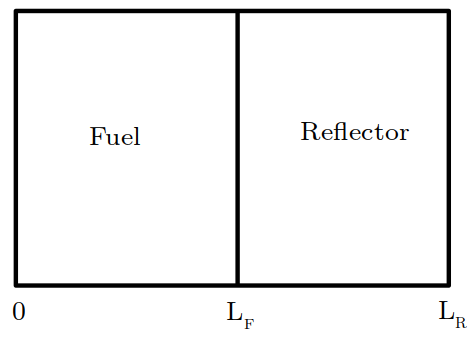
\includegraphics[width=3in]{2reg_geom}
    \caption{Geometry for Two-Region Problem.}
    \label{fg:2reg_geom}
  \end{figure}
  Boundary conditions on the horizontal surfaces (top/bottom) are reflective
  to reduce the problem to one-dimension. Other boundary conditions are given
  below.
  \begin{align}
    \phi'_F(0)&=0\\
    \phi_R(b)&=0\\
    D_F\phi'_F(a)&=D_R\phi'_R(a)
  \end{align}
  The material properties are specified below
  \begin{center}
  \begin{tabular}{c r r}
    & Fuel & Reflector\\
    $D$ & 1.2 & 0.7 \\
    $\Sigma_r$ & 0.02 & 0.015 \\
    $\nu \Sigma_f$ & 0.02 & 0 \\
    $q_{fixed}$ & 0 & 0
  \end{tabular}
  \end{center}
  The general form of the solution in the fueled region has the form 
  \[ \phi_F(x) = c_{1F} \cos(B_F x) + c_{2F} \sin(B_F x) \]
  Then, using the boundary condition $\phi'_F(0)=0$
  \begin{align}
    \phi_F(x) &= c_{1F} \cos(B_F x) + c_{2F} \sin(B_F x) \\
    \phi'_F(x) &= -B_F c_{1F} \sin(B_F x) + B_F c_{2F} \cos(B_F x) \\
    \phi'_F(0) &= 0\\
    &=B_F c_{2F}
  \end{align}
  Therefore, $c_{2F}=0$ and
  \begin{equation}
    \phi_F(x) = c_{1F} \cos(B_F x)
  \end{equation}
  Because this is an eigenvalue problem, $c_{1F}$ is arbitrary.
  
  Now for the solution in the reflector region. The solution has general form
  \begin{equation}
    \phi_R(x) = c_{1R} \cosh(B_R (x-a)) + c_{2R} \sinh(B_R (x-a))
  \end{equation}
  Treating the boundary condition $\phi_R(b)=0$
  \begin{align}
    \phi_R(x) &= c_{1R} \cosh(B_R (x-a)) + c_{2R} \sinh(B_R (x-a))\\
    \phi_R(b) &= 0 \\
    &= c_{1R} \cosh(B_R(b-a)) + c_{2R} \sinh(B_R(b-a))\\
    c_{1R} &= -c_{2R} \frac{\sinh(B_R(b-a))}{\cosh(B_R(b-a))}\\
    c_{1R} &= -c_{2R} \tanh(B_R(b-a))\\
    c_{2R} &= -c_{1R} \frac{1}{\tanh(B_R(b-a))} \label{eq:c2rnumber1}
  \end{align}
  Treating the current continuity boundary condition
  $D_F \phi'_F(a) = D_R \phi'_R(a)$.
  \begin{align}
    D_F \phi'_F(a) &= D_R \phi'_R(a) \\
    -D_F c_{1F} B_F \sin(B_F a) &= D_R B_R c_{2R} \\
    c_{2R} &= -\frac{D_F c_{1F} B_F \sin(B_F a)}{D_R B_R} \label{eq:c2rnumber2}
  \end{align}
  Treating the flux continuity boundary condition $\phi_F(a)=\phi_R(a)$.
  \begin{align}
    \phi_F(a)&=\phi_R(a) \\
    c_{1F} \cos(B_F a) &= c_{1R} \\
    c_{1R} &= c_{1F} \cos(B_F a) \label{eq:c1r}
  \end{align}
  Setting equations \eqref{eq:c2rnumber1} and \eqref{eq:c2rnumber2} equal.
  \begin{equation}
    - \frac{D_F c_{1F} B_F \sin(B_F a)}{D_R B_R} = -c_{1R} \tanh(B_R(b-a))
  \end{equation}
  Plugging in the the expression for $c_{1R}$ from \eqref{eq:c1r}
  \begin{align}
    - \frac{D_F c_{1F} B_F \sin(B_F a)}{D_R B_R} &=
      - \frac{c_{1F} \cos(B_F a)}{\tanh(B_R(b-a))}\\
    \frac{D_F B_F \sin(B_F a)}{D_R B_R} &= 
      \frac{\cos(B_F a)}{\tanh(B_R(b-a))} \\
    B_F \tan(B_F a) &= \frac{D_R B_R}{D_F \tanh(B_R(b-a))}
  \end{align}
  This is the most simplified solution. Unfortunately, there is no analytic
  expression for $B_F$. Therefore, a numeric solver must be used such as 
  MATLAB's \verb|vpasolve()| or a generic bisection/binary search. Because of
  the $\tan()$ function, the solution to $B_F$ is especially sensitive to the
  starting guess.
  
  Once $B_F$ is known, the problem is solved. By material definition, 
  ${B_R = \sqrt{\Sigma_{rR}/D_R}}$.
  \begin{align}
    \phi_F(x) &= \phi_0 \cos(B_F x)\\
    \phi_R(x) &= \phi_0 \cos(B_F a) \cosh(B_R (x-a)) 
      - \frac{D_F \phi_0 \sin(B_F a)}{D_R B_R} \sinh(B_R (x-a))\\
    \phi(x) &= H(x-a)\phi_R(x) + H(a-x)\phi_F(x)
  \end{align}
  Where $H(x)$ is the Heaviside step function.  
  
  The eigenvalue for this problem can be expressed for a known $B_F$. Similar 
  to \eqref{eq:keff1d} above, in this problem, for $a=50$, $b=100$
  \begin{align}
    B_F^2  &= 0.02559220482138791289 \\
    k_{eff} &= \frac{\nu\Sigma_{fF}}{D_F B_F^2 + \Sigma_{rF}} \\
    &= 0.96218825608052727105
  \end{align}
  
\section{One-Dimension, One-Group, Two-Region, Fixed-Source}
  This problem is similar to that described above except both regions are 
  non-fissile and there is a uniform fixed source in the problem. This will 
  draw on many previous equations.
  
  In this problem, material 1 is on the left and extends from 0 to $a$. 
  Material 2 is on the right and extends from $a$ to $b$. Boundary conditions 
  are $\phi(0)=\phi(b)=0$.
  
  The diffusion problem is written as \eqref{eq:onegroup} with 
  $\nu \Sigma_f =0$ and $q_{fixed}$ nonzero. Then, from \eqref{eq:particular},
  \begin{equation}
  	\phi_p = \frac{q_{fixed}}{\Sigma_r b}
  \end{equation}
  NOTE: This solution requires constant removal cross section in the two 
  materials. Otherwise, a different method for calculating the particular 
  solution must be used. The solution has general form similar to
  \eqref{eq:general}.
  \begin{align}
  	\phi &= \phi_p + \phi_1 H(a-x) + \phi_2 H(x-a) \\
    \phi_1 &= c_1 \cosh(B_1 x) + c_2 \sinh(B_1 x) \\
    \phi_2 &= c_3 \cosh(B_2 (x-a)) + c_4 \sinh(B_2 (x-a))
    \phi(0)&=\phi(b)=0
  \end{align}
  Where $B_i$ is the buckling coefficient for material $i$ given as
  \begin{equation}
    B_i = \sqrt{\Sigma_{ri} / D_i}
  \end{equation}
  
  Beginning with the boundary condition at $x=0$
  \begin{align}
    \phi(0) &= 0 \\
    &= \phi_p + c_1 \cosh(B_1 x) + c_2 \sinh(B_1 x) \\
    &= \phi_p + c_1\\
    c_1 &= -\phi_p \label{eq:bc_x0}
  \end{align}
  Next the boundary condition at $x=b$
  \begin{align}
    \phi(b) &= 0 \\
    &= \phi_p + c_3 \cosh(B_2 (b-a)) + c_4 \sinh(B_2 (b-a)) \\
    c_3 &= - \frac{\phi_p + c_4 \sinh(B_2(x-a))}{\cosh(B_2(b-a))} \\
    c_3 &= - \left(\frac{\phi_p}{\cosh(B_2(b-a))} + 
      c_4 \tanh(B_2(b-a))\right) \label{eq:bc_xb}
  \end{align}
  Next the interfacial boundary condition for conservation of flux
  $\phi(a^-)=\phi(a^+)$
  \begin{align}
    \phi(a^-) &= \phi(a^+) \\
    \phi_p - \phi_p \cosh(B_1 a) + c_2 \sinh(B_1 a) &= 
      \phi_p + c_3 \\
    c_3 &= c_2 \sinh(B_1 a) - \phi_p \cosh(B_1 a) \label{eq:bc_flux}
  \end{align}
  Next the interfacial boundary condition for conservation of current
  ${D_1 \phi'(a^-) = D_2 \phi'(a^+)}$
  \begin{align}
    D_1 \phi'(a^-) &= D_2 \phi'(a^+) \\
    D_1 (c_1 B_1 \sinh(B_1 a) + c_2 B_1 \cosh(B_1 a)) &=
      D_2 c_4 B_2 \\
    c_4 &= \frac{D_1 B_1}{D_2 B_2} (c_1 \sinh(B_1 a) + c_2 \cosh(B_1 a)) \\
    &= \frac{D_1 B_1}{D_2 B_2}(c_2 \cosh(B_1 a) - \phi_p \sinh(B_1 a))
      \label{eq:bc_current}
  \end{align}
  
  All of the coefficients have forward expressions given above except for 
  $c_2$. This will require significant algebra. Begin by setting 
  \eqref{eq:bc_xb} = \eqref{eq:bc_flux} and solve for $c_4$.
  \begin{align}
    - \left( \frac{\phi_p}{\cosh(B_2(b-a))} + c_4 \tanh(B_2 (b-a))\right)&=
      c_2 \sinh(B_1 a) - \phi_p \cosh(B_1 a) \\
    \phi_p \cosh(B_1 a) - \frac{\phi_p}{\cosh(B_2(b-a))} - 
      c_2 \sinh(B_1 a) &= c_4 \tanh(B_2 (b-a)) \\
    \phi_p \frac{\cosh(B_1 a)}{\tanh(B_2(b-a))} - 
      \frac{\phi_p}{\cosh(B_2(b-a))} 
      \frac{\cosh(B_2(b-a))}{\sinh(B_2(b-a))} - 
      c_2 \frac{\sinh(B_1 a)}{\tanh(B_2(b-a))} &= c_4\\
    \phi_p \left(\frac{\cosh(B_1 a)}{\tanh(B_2(b-a))} - \frac{1}
      {\sinh(B_2(b-a))} \right) - c_2 \frac{\sinh(B_1a)}{\tanh(B_2(b-a))} 
      &= c_4
  \end{align}
  Setting the above expression equal to \eqref{eq:bc_current} and finally 
  solve for $c_2$.
  \begin{align}
    \phi_p \left(\frac{\cosh(B_1 a)}{\tanh(B_2(b-a))} - 
      \frac{1}{\sinh(B_2(b-a))}\right) -
      c_2 \frac{\sinh(B_1 a)}{\tanh(B_2(b-a))} &=
      \frac{D_1 B_1}{D_2 B_2} \left( c_2 \cosh(B_1 a) - 
      \phi_1 \sinh(B_1 a)\right) \\
    \phi_p \left(\frac{\cosh(B_1 a)}{\tanh(B_2(b-a))} - 
      \frac{1}{\sinh(B_2(b-a))} \right) + 
      \frac{D_1 B_1}{D_2 B_2} \phi_p \sinh(B_1 a) &= 
      \frac{D_1 B_1}{D_2 B_2} c_2 \cosh(B_1a) + 
      c_2 \frac{\sinh(B_1a)}{\tanh(B_2(b-a))} \\
    \frac{\phi_p \left( \frac{\cosh(B_1a)}{\tanh(B_2(b-a))} - 
      \frac{1}{\sinh(B_2(b-a))} + 
      \frac{D_1 B_1}{D_2B_2} \sinh(B_1a) \right)}
      {\frac{D_1B_1}{D_2B_2} \cosh(B_1a) + 
      \frac{\sinh(B_1a)}{\tanh(B_2(b-a))}} &= c_2 \label{eq:c2}
  \end{align}
  Now, use equations \eqref{eq:bc_x0}, \eqref{eq:c2}, \eqref{eq:bc_flux}, and 
  \eqref{eq:bc_current} to solve for $c_1$ through $c_4$ respectively.
  
\section{Finite Cylinder, One Group, Criticality}
  The finite cylinder is an example of a truly three-dimensional problem with
  an analytic solution. This is a homogeneous cylinder with zero-flux boundary
  conditions on the edge of the cylinder. The cylinder has height $H$ and 
  radius $R$. The coordinates $r\in[0,R]$ and $z\in[0,H]$ where 
  $r=\sqrt{x^2+y^2}$.
  
  The solution method is by separation of variables into radial and axial 
  directions. Beginning with the axial direction. The diffusion equation can 
  be written
  \begin{equation} \label{eq:simplediffusion}
    \nabla^2 \phi(z) + B_z^2 \phi(z) = 0
  \end{equation}
  and has solution of the form
  \begin{equation} \label{eq:cyl_axial}
    \phi(z) = c_1 \cos(B_z z) + c_2 \sin(B_z z)
  \end{equation}
  Requiring $\phi(0)=\phi(H)=0$ yields $c_1=0$. Then $c_2$ is arbitrary and 
  the buckling condition is $B_zH=\pi$ and $B_z=\pi/H$.
  
  Moving on to the radial direction. The diffusion equation can be written.
  \begin{equation}
    \nabla^2 \phi(r) + B_r^2 \phi(r) = 0
  \end{equation}
  Noting the radial coordinates.
  \begin{align}
    \frac{1}{r} \frac{\partial}{\partial r} \left( r \frac{\partial \phi}
      {\partial r} \right) + B_r^2 \phi &= 0 \\
    \frac{\partial}{\partial r} \left( r \frac{\partial \phi}{\partial r}
      \right) + B_r^2 \phi &= 0
  \end{align}
  Noting the product rule of differentiation.
  \begin{align}
    r \frac{\partial^2 \phi}{\partial r^2} + \frac{\partial \phi}
      {\partial r} + B_r^2 r \phi &= 0 \\
    \frac{\partial^2 \phi}{\partial r^2} + \frac{1}{r} \frac{\partial \phi}
      {\partial r} + B_r^2 \phi &= 0 \label{eq:besselequation}
  \end{align}
  Noting equation \eqref{eq:besselequation}, Lewis Appendix B shows the 
  equation has solution of the form
  \begin{equation} \label{eq:cyl_radial}
    \phi(r) = c_3 J_0(B_r r) + c_4 Y_0(B_r r)
  \end{equation}
  Where $J_0$ is the Bessel function of the first kind, zeroth order and $Y_0$
  is the Bessel function of the second kind, zeroth order. Requiring the flux
  to be finite at $r=0$ requires $c_4=0$ as 
  $\lim_{r\rightarrow0} Y_0(r)=-\infty$. Again, $c_3$ is arbitrary. Zero flux 
  boundary conditions requires $B_r R=\alpha_0$ where $\alpha_0$ is the first 
  zero of the $J_0$ function and $\alpha_0 \approx 2.4048$. Then 
  $B_r=\alpha_0/R$.
  
  Combining the radial expression \eqref{eq:cyl_radial} and the axial 
  expression \eqref{eq:cyl_axial} yields the final expression for the flux.
  \begin{align} \label{eq:cyl_flux}
    \phi(r,z) &= J_0(B_r r) \sin(B_z z) \\
    &= J_0(r \alpha_0 / R) \sin(z \pi / H)
  \end{align}
  Plugging \eqref{eq:cyl_flux} into the diffusion equation will yield the 
  buckling/criticality condition.
  \begin{equation}
    -D \left( \frac{1}{r} \frac{\partial}{\partial r} \left( r 
      \frac{\partial \phi}{\partial r} \right) + \frac{\partial^2 \phi}
      {\partial z^2} \right) + \Sigma_r \phi = \frac{1}{k_{eff}} \nu 
      \Sigma_f \phi
  \end{equation}
  Beginning with the differentiation terms for simplicity. Axial 
  differentiation is straight-forward and presented below.
  \begin{equation}
    \frac{\partial^2 \phi}{\partial z^2} = -B_z^2 J_0(B_r r) \sin(B_z z)
  \end{equation}
  Radial differentiation must account for the radial geometry and is more 
  complex. First, note the following derivative relationship of the zeroth
  order Bessel function.
  \begin{equation} \label{eq:deriv_bessel0}
    \frac{d}{dr} J_0(\alpha r) = - \alpha J_1(\alpha r)
  \end{equation}
  \begin{align}
    \frac{\partial \phi}{\partial r} &= -B_r \sin(B_z z) J_1(B_r r) \\
    r \frac{\partial \phi}{\partial r} &= -B_r \sin(B_z z) r J_1 (B_r r) 
  \end{align}
  Note the additional derivative relation for the general Bessel function.
  \begin{equation} \label{eq:deriv_besseln}
    \frac{d}{dr} J_n(r) = \frac{1}{2} \left( J_{n-1}(r) - J_{n+1}(r)\right)
  \end{equation}
  Evaluating the rest of the cylindrical derivative using
  \eqref{eq:deriv_besseln} and the product rule.
  \begin{align}
    \frac{\partial}{\partial r} \left( r \frac{\partial \phi}{\partial r}
      \right) &= -B_r \sin(B_z z) \left(J_1(B_r r) + \frac{1}{2} B_r r \left(
      J_0(B_r r) - J_2(B_r r) \right) \right) \\
    \frac{1}{r} \frac{\partial}{\partial r} \left(r 
      \frac{\partial \phi}{\partial r} \right) &=
      -B_r \sin(B_z z) \left(\frac{1}{r} J_1(B_r r) + \frac{1}{2} B_r \left(
      J_0(B_r r) - J_2(B_r r) \right) \right)
  \end{align}
  Finally, plugging the expression for the Laplacian of the flux back into the
  diffusion equation.
  \begin{multline}
    D \left( B_r \sin(B_z z) \left( \frac{1}{r} J_1(B_r r) + \frac{1}{2} B_r
    \left( J_0(B_r r) - J_2(B_r r) \right) \right) + B_z^2 J_0(B_r r) \sin(B_z
    z) \right) + \\
    \Sigma_r J_0(B_r r) \sin(B_z z) \\
    = \frac{1}{k_{eff}} \nu
    \Sigma_f J_0(B_r r) \sin(B_z z)
  \end{multline}
  Dividing through by $\sin(B_z z)$.
  \begin{multline}
    D \left( B_r \left( \frac{1}{r} J_1(B_r r) + \frac{1}{2} B_r
    \left( J_0(B_r r) - J_2(B_r r) \right) \right) + B_z^2 J_0(B_r r) \right)+\\
    \Sigma_r J_0(B_r r) = \frac{1}{k_{eff}} \nu \Sigma_f J_0(B_r r) 
  \end{multline}
  Dividing through by $J_0(B_r r)$ and expanding some terms.
  \begin{align}
    D \left( B_r \left( \frac{1}{r} \frac{J_1(B_r r)}{J_0(B_r r)} + 
      \frac{1}{2} \left(B_r - \frac{J_2(B_r r)}{J_0(B_r r)} \right) \right) 
      + B_z^2 \right)+ \Sigma_r &= \frac{1}{k_{eff}} \nu \Sigma_f \\
    D \left( \frac{1}{r} B_r \frac{J_1(B_r r)}{J_0(B_r r)} + \frac{B_r^2}{2} -
      \frac{B_r^2}{2} \frac{J_2(B_r r)}{J_0(B_r r)} + B_z^2 \right) + \Sigma_r&=
      \frac{1}{k_{eff}} \nu \Sigma_f  \\
    \frac{1}{r} B_r \frac{J_1(B_r r)}{J_0(B_r r)} + \frac{B_r^2}{2} -
      \frac{B_r^2}{2} \frac{J_2(B_r r)}{J_0(B_r r)} + B_z^2 + 
      \frac{\Sigma_r}{D} &= \frac{1}{k_{eff}} \frac{\nu \Sigma_f}{D}\\
    \frac{1}{J_0(B_r r)} \frac{B_r^2}{2} \left(\frac{1}{r} \frac{2}{B_r} 
      J_1(B_r r) - J_2(B_r r) \right) + \frac{B_r^2}{2} + B_z^2 + 
      \frac{\Sigma_r}{D} &= \frac{1}{k_{eff}} \frac{\nu \Sigma_f}{D}
  \end{align}
  Note the Bessel function recursion relationship.
  \begin{equation} \label{eq:bessel_recursion}
    J_{n+1}(\alpha r) + J_{n-1}(\alpha r) = \frac{2n}{\alpha r} J_n(\alpha r)
  \end{equation}
  Using \eqref{eq:bessel_recursion} the term above is simplified.
  \begin{align}
    \frac{1}{J_0(B_r r)} \frac{B_r^2}{2} \left( J_0(B_r r) \right) + 
      \frac{B_r^2}{2} + B_z^2 + \Sigma_r &= \frac{1}{k_{eff}} 
      \frac{\nu \Sigma_f}{D} \\
    B_r^2 + B_z^2 + \frac{\Sigma_r}{D} &= \frac{1}{k_{eff}} \frac{\nu \Sigma_f}
      {D}
  \end{align}
  Now, an expression for the eigenvalue can be written.
  \begin{align}
    k_{eff} &= \frac{\nu \Sigma_f}{D(B_r^2 + B_z^2) + \Sigma_r} \\
    &= \frac{\nu \Sigma_f}{D\left(\left(\frac{\alpha_0}{R}\right)^2 + 
      \left(\frac{\pi}{H}\right)^2 \right) + \Sigma_r}
  \end{align}
  NOTE: the shape of the boundary is \textbf{extremely} important for this 
  problem. Therefore
  the mesh must be regenerated from scratch for each 
  refinement, rather than simply splitting nodes.
  
